\documentclass{article}
% ready for submission
\usepackage[preprint, nonatbib]{neurips_2023}
\usepackage{biblatex} %Imports biblatex package
\addbibresource{sample.bib} %Import the bibliography file
\usepackage{graphicx}
\usepackage{algorithm2e}
\usepackage{hyperref}

% to compile a preprint version, e.g., for submission to arXiv, add add the
% [preprint] option:
%\usepackage[preprint]{neurips_2023}


% to compile a camera-ready version, add the [final] option, e.g.:
%     \usepackage[final]{neurips_2023}


% to avoid loading the natbib package, add option nonatbib:
%    \usepackage[nonatbib]{neurips_2023}


\usepackage[utf8]{inputenc} % allow utf-8 input
\usepackage[T1]{fontenc}    % use 8-bit T1 fonts
\usepackage{hyperref}       % hyperlinks
\usepackage{url}            % simple URL typesetting
\usepackage{booktabs}       % professional-quality tables
\usepackage{amsfonts}       % blackboard math symbols
\usepackage{nicefrac}       % compact symbols for 1/2, etc.
\usepackage{microtype}      % microtypography
\usepackage{xcolor}         % colors
\usepackage{float}


\title{Image Recovery From Underexposed Photographs Using Generative Models}

\author{
  Moises Lopez \\
  Department of Electrical & Computer Engineering \\
  University of Califonia San Diego \\
  % La Jolla, CA 92093 \\
  \texttt{mlopezme@ucsd.edu} \\
  % examples of more authors
  \And
  Sepehr Aiden Bostan \\
  Department of Electrical & Computer Engineering \\
  University of Califonia San Diego \\
  % La Jolla, CA 92093 \\
  \texttt{sbostanb@ucsd.edu} \\
  \And
  Yiteng Zhao \\
  Department of Electrical & Computer Engineering \\
  University of Califonia San Diego \\
  % La Jolla, CA 92093 \\
  \texttt{yiz097@ucsd.edu}
}


\begin{document}


\maketitle
\begin{abstract}
  Low light imagery has been a persistent challenge in fields like photography, computer vision, and feature detection. To address this problem, probabilistic methods and deep generative models such as GANs have emerged as promising solutions. In this paper, we present our approach to recovering underexposed images using GAN-based techniques, while also addressing the shortcomings of existing methods. Our proposed approach improves the quality of recovered images, making them more visually appealing and useful in various applications such as object detection in low light using cameras or simply photography in extremely dark conditions.
\end{abstract}

\section{Github Repository}

Please check out our project on GitHub: \href{https://github.com/mdlopezme/ece285_project_deep.git}{https://github.com/mdlopezme/ece285\textunderscore project\textunderscore deep.git}.


\section{Introduction}
\subsection{What research problem are we trying to solve?}
Social media and computer vision applications demand high-quality images, but current CMOS sensors used in cameras and smartphones struggle to perform well in challenging lighting conditions due to physical limitations. Low levels of photons captured by CMOS pixels result in dark, under-exposed images that are difficult for both computer analysis and human perception. Traditional physical methods such as enlarging pixels, aperture or increasing ISO can improve the Signal-to-Noise ratio, but at the cost of resolution, depth of field, or noise in the image. Therefore, our research aims to develop a better computational approach using a probabilistic neural network model to recover under-exposed images while maintaining their sharpness, color accuracy, and cleanliness.

\subsection{Why is this problem important?}
The potential of solving this problem can extend from mere convenience to saving lives. For example, in computer vision and autonomous vehicles, instead of using lidars in low light conditions we can simply use cameras for object detection and obstacle avoidance. Similarly, in search and rescue operations, a similar method can be used. In radiation imagery such as x-ray images used in the medical field, underexposed pixels can result in a loss of crucial details, potentially hiding a small tumor or other irregularities that would otherwise be detected by medical professionals. On the other hand, in photography, underexposed images can be recreated with higher brightness, which can merely be convenient for people.
\section{Related Works}

The literature has thoroughly examined the computational processing of low-light images. We will give a brief overview of the methods currently available.

\subsubsection{Convolutional Neural Networks} 
Researchers have explored the use of deep neural networks for extreme low-light imaging, but the approach has limitations and shortcomings. One issue is that the convolutional network\cite{LearningToSeeInTheDark} is individually tuned for each camera sensor, requiring cross-sensor generalization to be effective across different cameras. The hyper-parameters of the network, such as amplification factors, also need to be manually tuned, indicating the need for an auto ISO feature to improve efficiency. Additionally, the absence of HDR tone mapping and dynamic objects in the dataset limits the network's ability to enhance such images. Artifacts in the final image could also potentially be reduced. Finally, the long processing time of 0.38-0.66 seconds per image could be problematic for real-time applications. These limitations need to be addressed to improve the practicality and effectiveness of deep neural networks for image enhancement.

\subsubsection{Low-light image enhancement.}

There are different techniques for image enhancement, including histogram equalization and gamma correction. Histogram equalization involves balancing the histogram of the entire image, while gamma correction increases the brightness of dark regions and compresses bright pixels. More advanced techniques involve global analysis and processing, such as the inverse dark channel prior, wavelet transform \cite{AutomaticContrastEnhancement}, Retinex model\cite{retinex}, and illumination map estimation\cite{illumest}. However, these techniques typically assume that the images already have a good representation of the scene content.

However, we are focusing on extreme low-light imaging, which is characterized by high levels of noise and color distortion that exceed the capabilities of current enhancement pipelines.

\section{Methodology}
%\subsection{Proposed a solution for solving this problem}
We propose a generative network model that is designed to analyze and sample from the distribution of under-exposed images, and generate well-exposed images for comparing against the discriminate network using CNNs with ground truth as input. We will delve deeper into the structure of the network and steps later.
% \section{Novelty and significance of our solution}
% Our solution increases the quality and usability of underexposed images which are common in various applications. As mentioned before the potential of solving this problem can extend from mere convenience to saving lives.

\section{Method}
% \subsection{The Pipeline}
% The present study aims to use a dataset comprising of underexposed images, which are paired with corresponding longer exposure images that serve as the ground truth. Specifically, the See-In-The-Dark (SID) dataset, consisting of approximately 5,000 high-resolution images will be utilized. The SID dataset comprises of 5094 raw short-exposure images, each paired with a reference long-exposure image. It is important to note that each long-exposure image is paired with multiple short-exposure images. The dataset contains both indoor and outdoor images, indoor images were set in a specially dark environment. The images are taken using two different cameras. the first is a Sony camera that has a full-frame Bayer sensor and the second is a Fujifilm camera that has an APS-C X-Trans sensor setup in a way to reduce the noise for the long exposure images as much as possible.

% To achieve our objective of direct single-image processing of fast low-light images, we propose to utilize end-to-end learning. This will be accomplished through training a variational autoencoder (VAE) in conjunction with a convolutional neural network (ConvNet) proposed in paper SIG \cite{LearningToSeeInTheDark} to perform the entire image processing pipeline. The VAE will be responsible for providing artistic enhancements to the images, while the ConvNet will be utilized to recover the high frequency details from the low signal-to-noise ratio (SNR) image. The ConvNet will be implemented using U-Net architecture. % More explaination on U-Net

% The output from the VAE and the ConvNet will be summed together and then passed through a discriminator network. 
\begin{figure}[H]
  \centering
  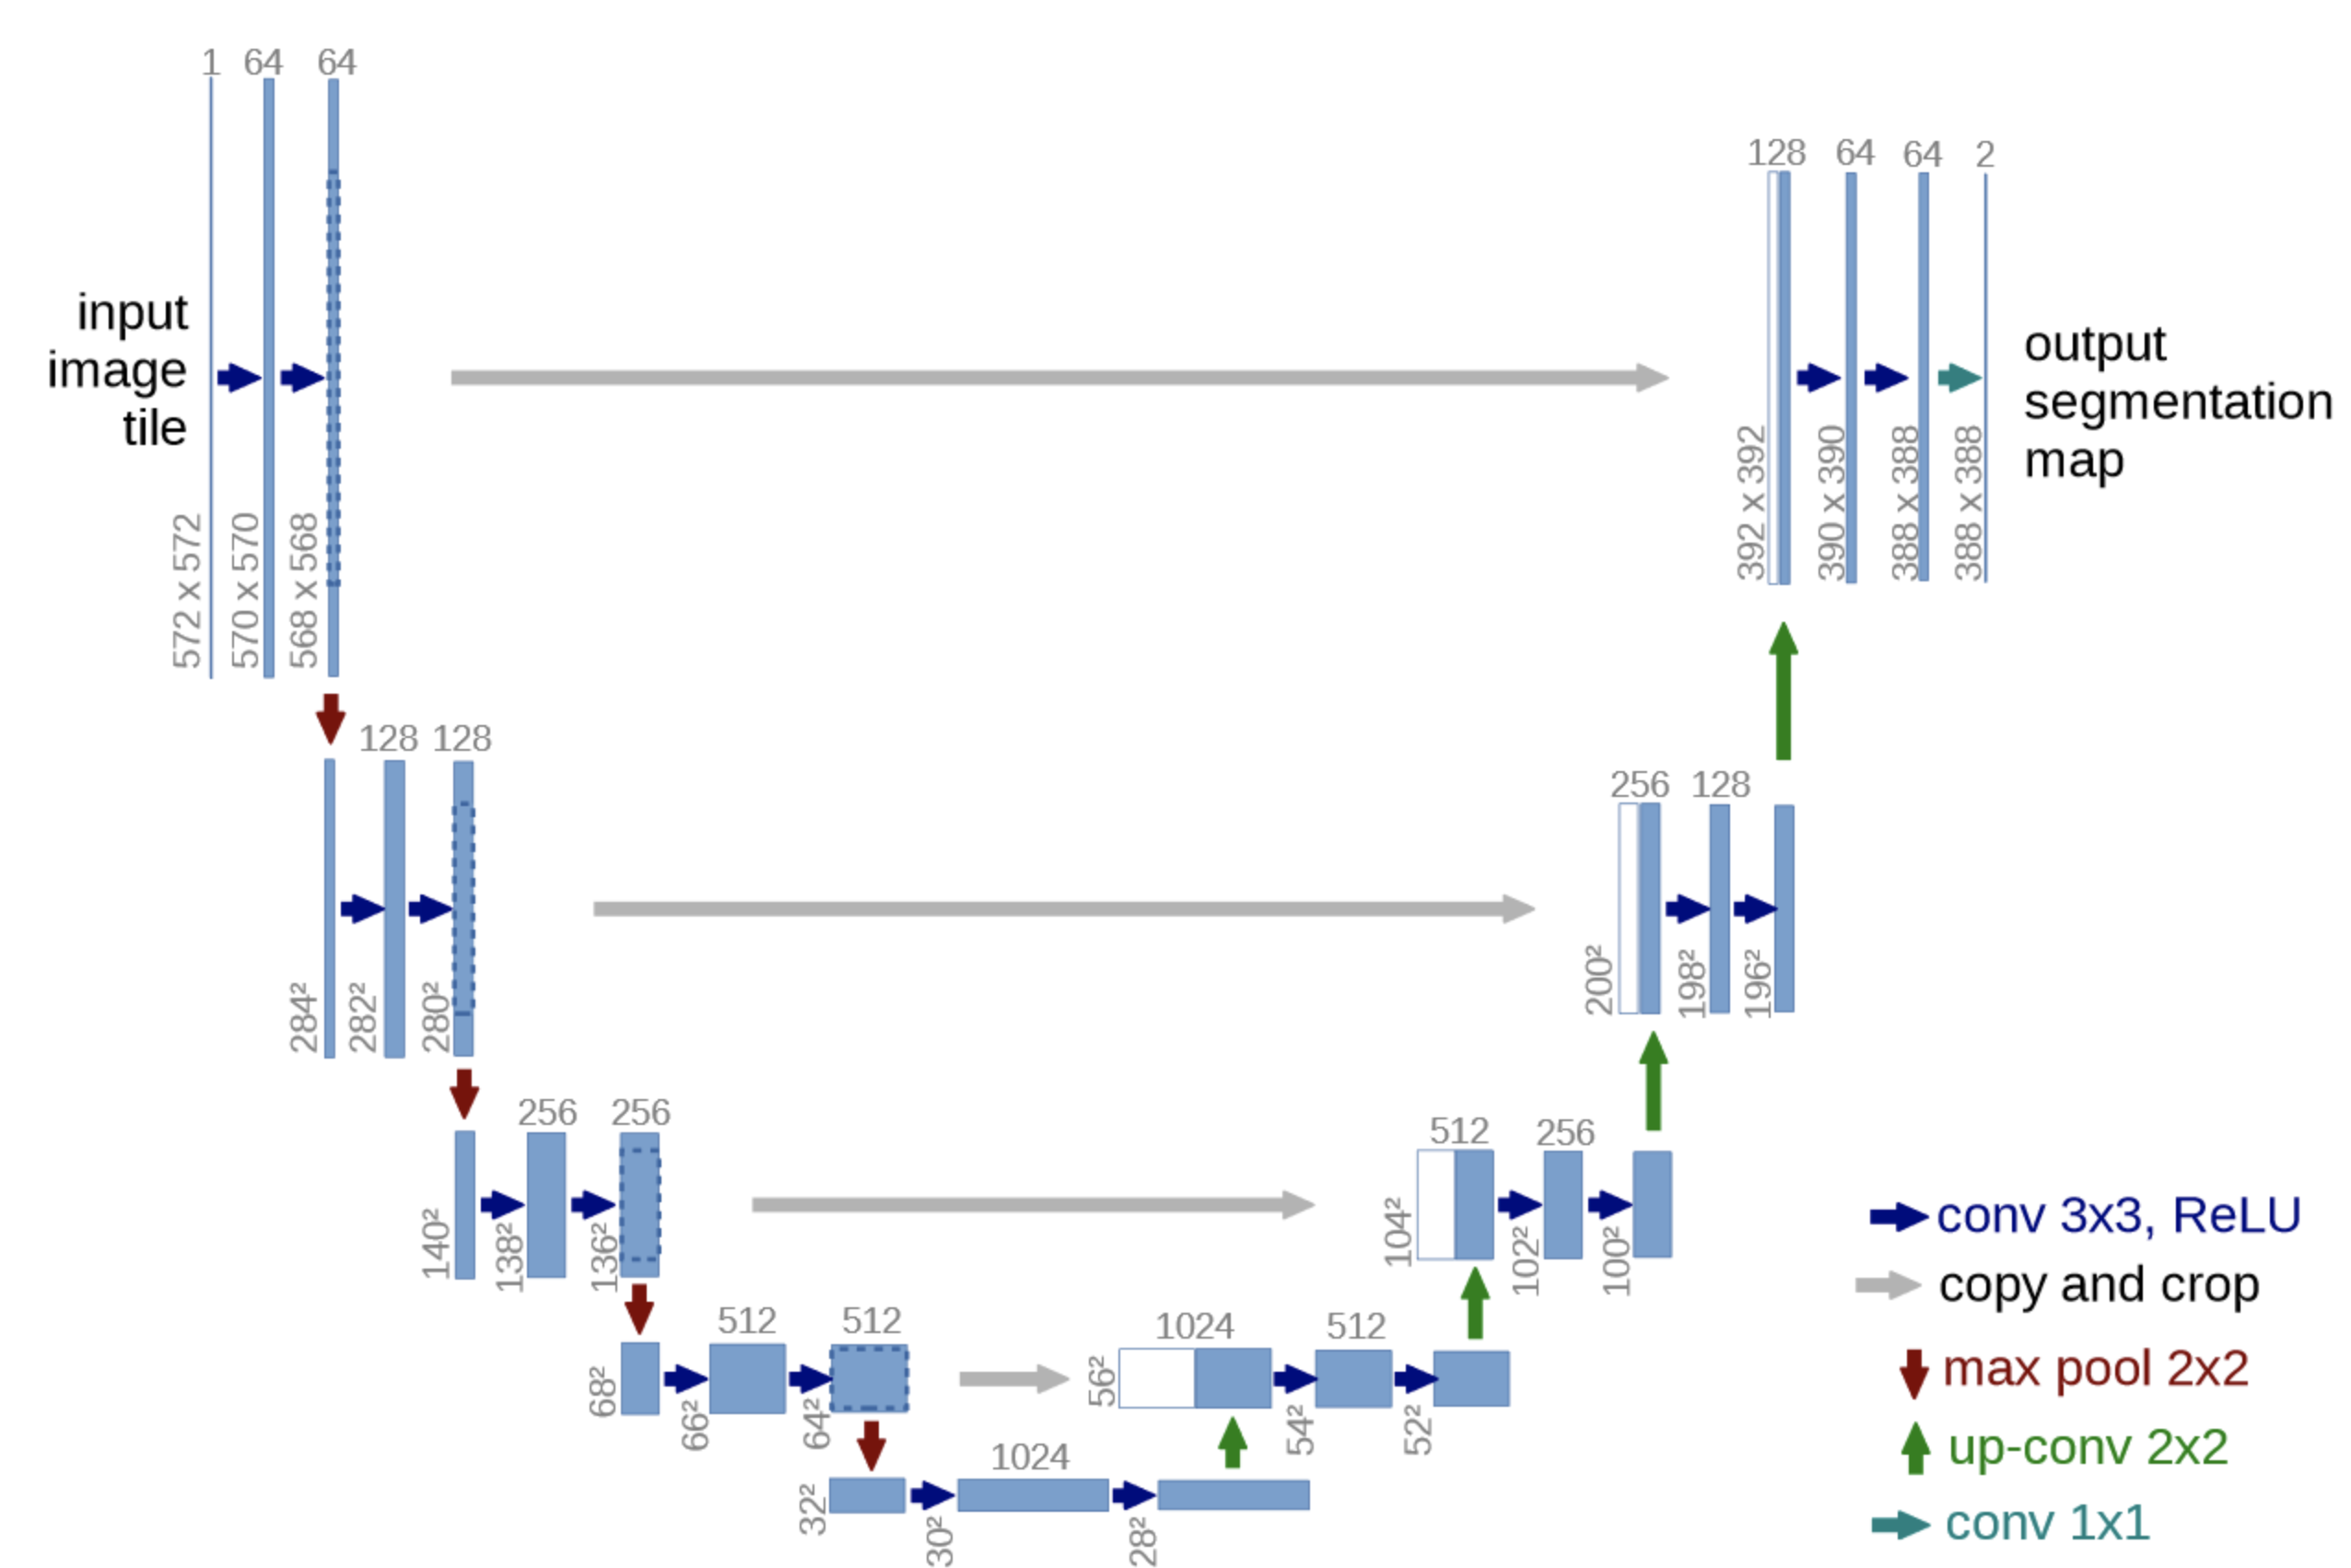
\includegraphics[width=\textwidth]{UnetArch.png}
\end{figure}
\subsection{Training}
The training process for the proposed image enhancement method consists of several key steps, including data pre-processing,
model training, optimization, and learning rate scheduling. This section presents a comprehensive overview of the training procedure.

\subsubsection{Data Preprocessing}
Prior to training the model, the training dataset undergoes essential pre-processing steps. Random cropping is employed to extract image
patches from the input data, ensuring diversity in the training samples. The process involves randomly selecting starting positions
within the images and cropping them to a specified size. Additionally, specific pre-processing techniques are applied to align the input images with the target ground truth
images, such as normalization and data format conversions. These pre-processing steps aim to facilitate effective learning and 
improve the model's ability to generalize the unseen data. 

\subsubsection{Model Training and Optimization}
The training step encompasses the iterative process of optimizing the model's parameters based on the available training data.
During training, the model is presented with preprocessed images. The output of the network is then supervised under the ground truth and compared against them. This comparison is used to
compute a loss metric that quantifies the discrepancy between the model's prediction and the desired outputs. The optimization
process involves minimizing  this loss by adjusting the model's parameters through backpropagation and gradient-based optimization
techniques. Specifically, the gradients are computed with respect to the model's parameter using the chain rule, and an optimization algorithm
is employed to update the parameters in the direction that reduces the loss. This iterative optimization process incrementally refines
the model's capabilities and enables it to better approximate the desired image enhancement function.

% \subsubsection{Learning Rate Scheduling}
% The learning rate, a hyperparameter controlling the step size during optimization, plays a crucial role in determining the convergence speed
% and stability of the training process. A carefully chosen learning rate schedule can significantly impact the model's performance. In
% our training procedure, a learning rate scheduler is employed to dynamically adjust the learning rate throughout the training process. 
% In our approach, we employ the StepLR scheduler from torch.optim.lr\textunderscore scheduler module with a step size of 10 and a gamma factor of 0.8. This 
% means that after every 10 training steps, the learning rate is multiplied by 0.8. By adapting the learning rate according to this schedule,
% the scheduler enables the model to navigate the optimization landscape more effectively, potentially avoiding sub-optimal solutions and achieving
% better convergence.

% The combination of data pre-processing, model training, optimization, and learning rate scheduling forms a coherent training framework for this
% image enhancement task. This frameworks aims to improve the model's ability to enhance dark images by comparing them against ground truth
% long exposure images. BY iteratively optimizing the model's parameters and adjusting the learning rate according to the especified schedule, we
% aim to achieve a well-trained model capable of accurately enhancing dark images and preserving important image details.
\subsubsection{Loss Function}
We used L1 loss to calculate the loss for each iteration in network model output. The choice of L1 loss function is motivated by its ability to preserve image details and promote spatially consistent enhancements. Unlike other loss functions, such the L2 loss (mean squared error), the L1 loss is less sensitive to outliers and encourages sparser errors. This property is beneficial in the context of image enhancement, where preserving fine details and avoiding over-smoothing are desirable.
\section{Algorithm}

Algorithm 1 presents the training procedure for the proposed image enhancement method using the U-Net architecture. The algorithm outlines the steps involved in training the model and optimizing its parameters.

\begin{algorithm}[H]
  \SetAlgoLined
  \KwIn{Training dataset: images taken in the dark (input) and corresponding ground truth long exposure images (target)}
  \KwIn{Hyperparameters: learning rate, step size, gamma}
  \KwOut{Trained U-Net model}
  
  \textbf{Preprocessing:}
  Randomly crop input images and corresponding ground truth images to extract image patches of a specified size.
  Apply normalization and data format conversions to align the input images with the target ground truth images.
  
  \textbf{Initialize Model:}
  Create an instance of the U-Net model.
  Set the initial model parameters.
  
  \textbf{Initialize Optimizer:}
  Select an optimization algorithm, such as Adam.
  Initialize the optimizer with the model parameters and a specified learning rate.
  
  \textbf{Initialize Learning Rate Scheduler:}
  Configure the learning rate scheduler with the selected scheduler (e.g., StepLR).
  Set the step size and gamma values according to the predefined parameters (step\_size = 10, gamma = 0.8).
  
  \textbf{Training Loop:}
  \Repeat{convergence or a predefined number of iterations}{
    \textbf{Model Training:}
    Set the model in training mode.
    Clear the gradients of the optimizer.
    Retrieve a batch of cropped input images and corresponding ground truth images.
    Transfer the data to the device (e.g., GPU).
    Perform additional preprocessing steps, such as packing the raw images (if applicable) and adjusting exposure ratios.
    Pass the preprocessed input images through the U-Net model to obtain the output predictions.
    Calculate the loss between the predictions and the ground truth images using a suitable loss function (e.g., L1 loss).
    Backpropagate the gradients through the model to compute the gradients with respect to the model parameters.
    Update the model parameters by taking an optimization step using the optimizer.
    
    \textbf{Learning Rate Scheduling:}
    Adjust the learning rate according to the predefined schedule.
    Update the learning rate based on the step size and gamma values.
    Modify the optimizer's learning rate using the updated value.
  }
  
  \textbf{Output:}
  Return the trained U-Net model.
  
  \caption{Training the U-Net for Image Enhancement}
\end{algorithm}

The training algorithm follows a standard procedure for training deep neural networks. It involves preprocessing the data, initializing the model, optimizer, and learning rate scheduler, and then iteratively updating the model parameters while adjusting the learning rate. By optimizing the model with respect to the loss function, the algorithm aims to train the U-Net to accurately enhance dark images when compared to their corresponding ground truth long exposure images.



\section{Theory} %change this Unet-VAE -> UNet-GAN
% \begin{figure}[h]
%   \centering
%   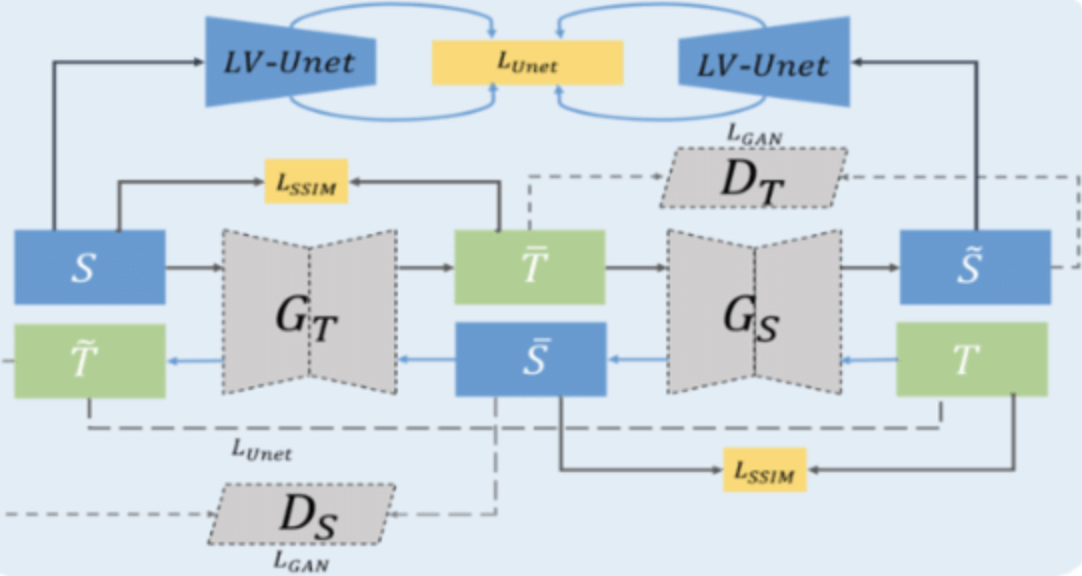
\includegraphics[width=\textwidth]{UnetGanArchitecture.png}
% \end{figure}

The proposed method for direct single-image processing of fast low-light images involves the use of advanced deep learning techniques, specifically, a U-Net architecture. The U-Net is a convolutional neural network that has been shown to be effective in image segmentation \cite{UNetBasedMedicalImageSegmentation} and other image processing tasks. 

In this approach, the U-net is used to improve the image quality of underexposed images while recovering the ground truth data. The U-net is trained on a dataset of paired under-exposed and well-exposed images, where the low-light image is the input, and the highlight image is the ground truth. The U-Net learns to map the low-light image to the high-light image, recovering the lost information due to the low signal-to-noise ratio.

To further enhance the overall image quality, the U-Net is trained in conjunction with a generative model, such as a variational autoencoder (VAE). The VAE is used to provide artistic enhancements to underexposed images, such as adjusting the brightness, contrast, and color saturation. The VAE is trained on a large dataset of high-quality images and then used to enhance the underexposed images.

To optimize the overall image quality, the U-Net and VAE are trained in parallel, allowing the VAE to improve the overall appearance of the image, while the U-Net improves the accuracy of the image. The loss function used to train the model combines the objectives of the U-Net and VAE, encouraging the model to produce high-quality images that are close to the ground truth.

The model is trained on a dataset of paired short-exposure and long-exposure images, allowing the model to learn from multiple examples of the same ground truth data. Finally, the output of the U-Net and VAE are combined and evaluated using a discriminator network to ensure that the final image is of high quality.
\section{Additional Experiments}
\subsection{UNet with Generative Adversarial Network}
We experiment on improving the UNet structure proposed in SID paper \cite{LearningToSeeInTheDark} by attaching a discriminator network and provide adversarial loss to the generator, UNet. Since we are using UNet as the generator, we choose UNet as our discriminator in order to lower the difference between generator and discriminator. The UNet discriminator architecture and losses are adapted from another paper \cite{unetd}. % Explain on UNet Discriminator
\subsection{U-UNet -- Double UNet with skip-z}
We want to improve on the washed-out color of the output from our baseline model, therefore we experiment on whether chaining another model on top of the pre-trained baseline model will help with improving the color. We called this model U-UNet because we not only feed the output from the previous UNet, we also use skip connections between the upsampling layer of previous UNet and downsampling layer of next UNet model, similar to the skip connection from downsampling layer to upsampling layer. 
\subsection{Deeper UNet}
% WHAT DID you observed with a deeper U-NET? Worse performance, not converging, loss cannot propagate to deeper layer
% WHERE THE FUCK IS SEPHER!>!>!??!!??!?!?! PUB
We also experimented with deep U-net architectures, aiming to leverage the increase capacity of the model to capture more complex features and improve overall performance. However, we observed worse performance compared to baseline U-Net mode, with the models struggling to converge and the loss being unable to effectively propagate through the deeper layers. This limitation suggest simply increasing the depth of the U-Net may not necessarily lead to improved performance. Further investigations are necessary to identify the underlying causes of the issue and explore potential strategies to overcome it. 

\subsection{UNet with Attention}
Another approach we explored to enhance our image restoration efforts was to utilize U-net models with attention mechanism. By incorporating attention mechanism into the U-Net architecture, we aimed to improve the model's ability to focus on relevant image features. This attention mechanism allows the network to dynamically allocate its resources to important regions, effectively enhancing the model's ability to capture fine details and improve overall image quality. Through our experimentation, we observed that U-Net with attention demonstrated promising results, showcasing improved restoration performance compared to the baseline U-Net model. However, despite visual improvements achieved, we observed that the numerical results were slightly worse compared to the baseline U-Net model.

\section{Results}
The following is a summary of our results.

\subsection{Test Results}

%Unet Results
\begin{figure}[H]
  \centering
  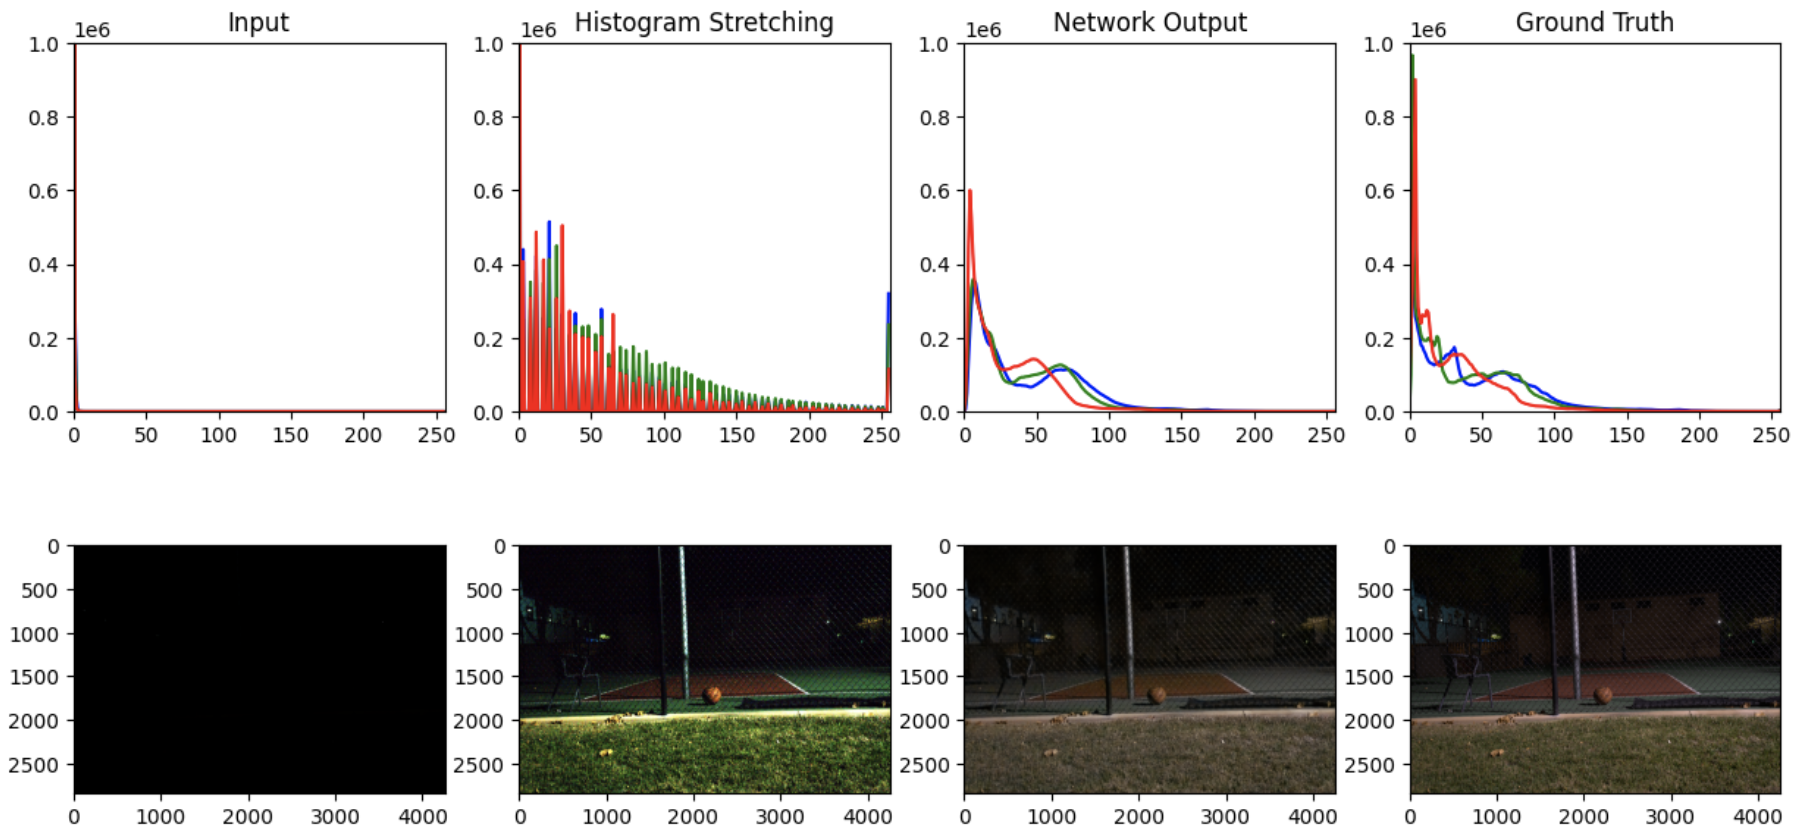
\includegraphics[width=\textwidth]{Result1Unet1.png}
  \caption{Sample output from Baseline Model}
\end{figure}
\begin{figure}[H]
  \centering
  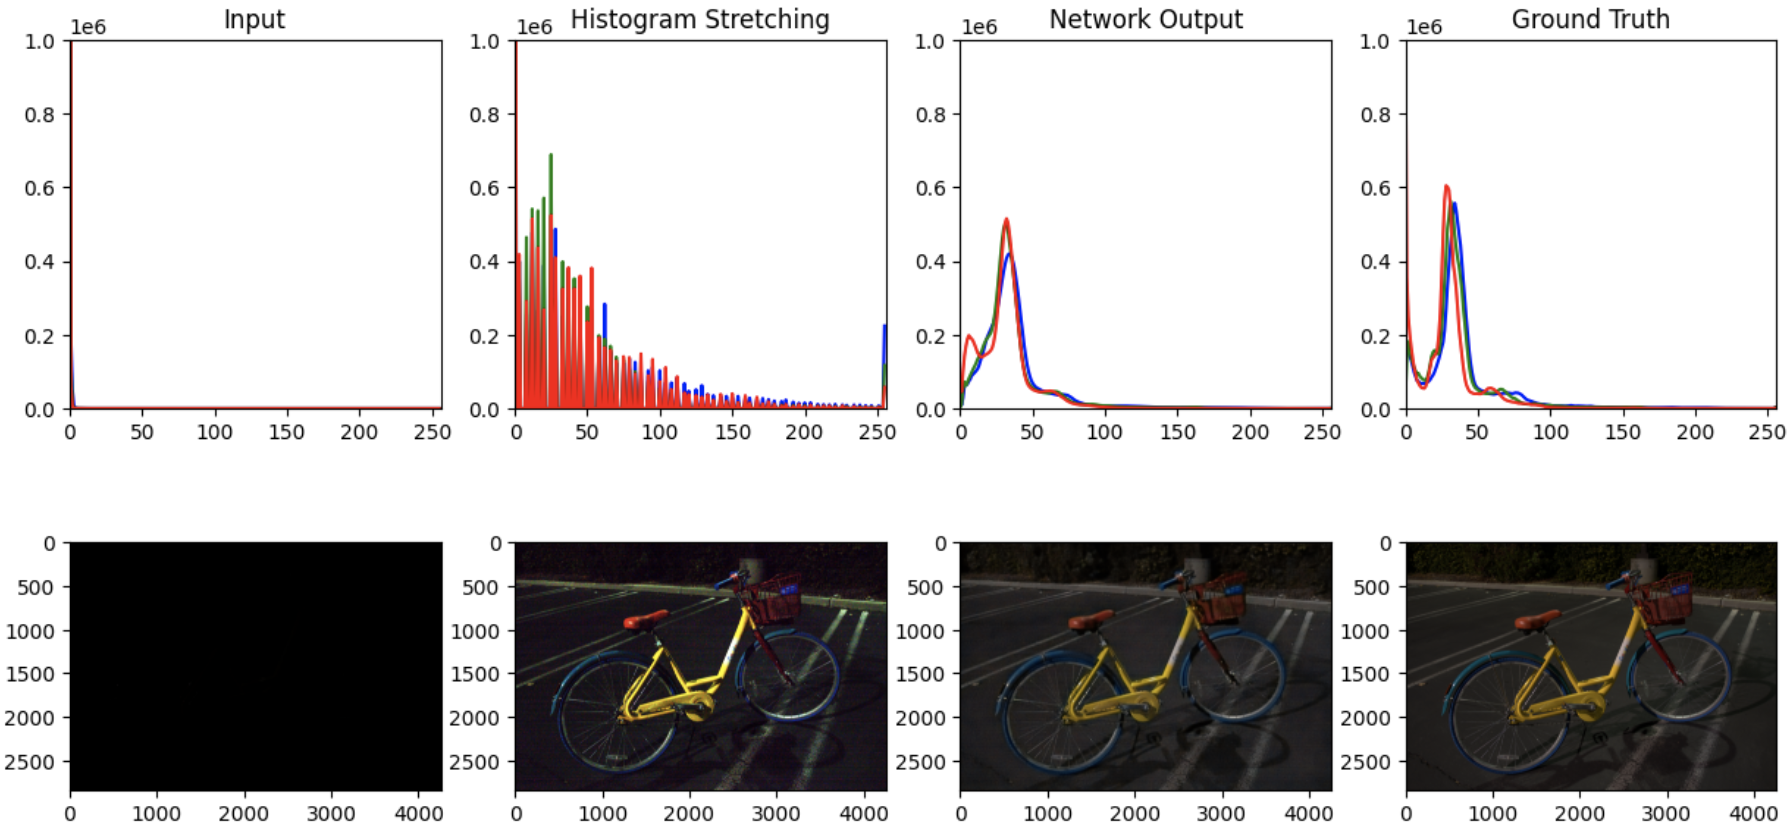
\includegraphics[width=\textwidth]{Result2Unet1.png}
  \caption{Sample output from Baseline Model}
\end{figure}
\begin{figure}[H]
  \centering
  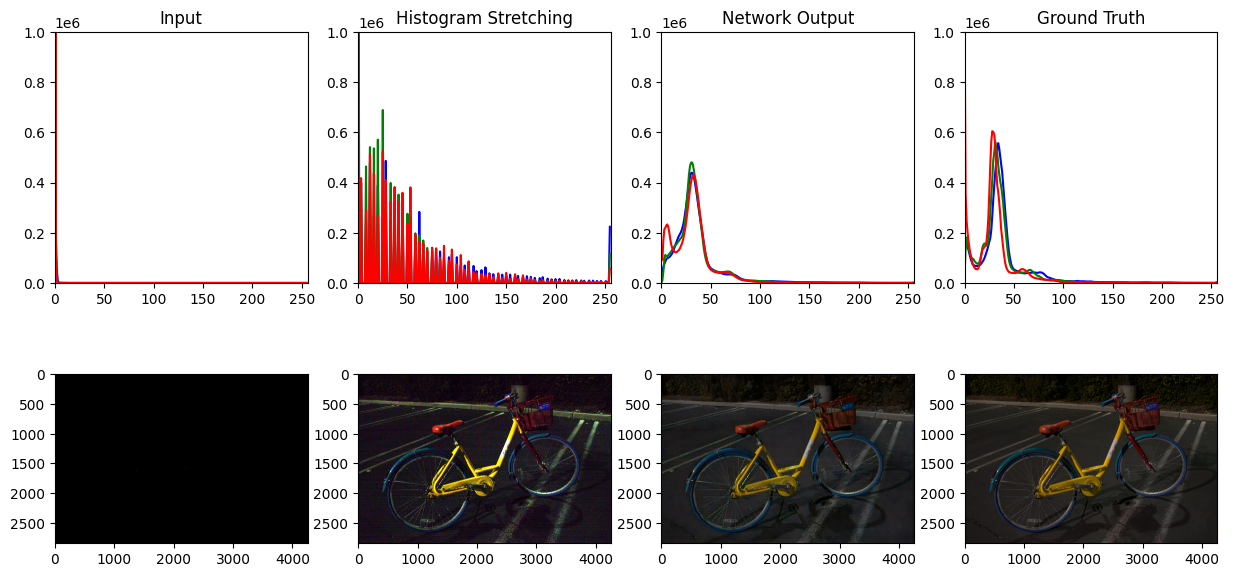
\includegraphics[width=\textwidth]{Result1UnetGAN.png}
  \caption{Sample output from UNet GAN Model}
\end{figure}
\begin{figure}[H]
  \centering
  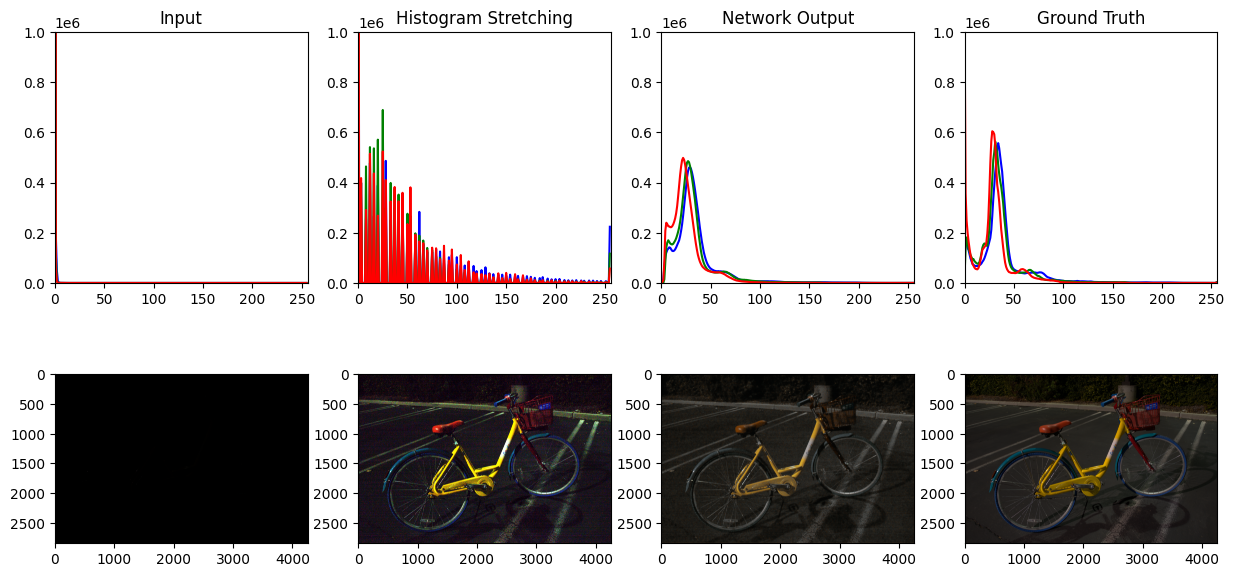
\includegraphics[width=\textwidth]{Result1UnetAttn.png}
  \caption{Sample output from UNet Attention Model}
\end{figure}



\subsection{Evaluation}
We evaluate the performance of models that produces acceptable results using PSNR, Peak Signal-to-Noise Ratio, and SSIM, Structural Similarity Index Measure: 
\begin{table}[H]
    \centering
    \begin{tabular}{|c|c|c|}
        \hline
        Model & PSNR & SSIM\\
        \hline
        Baseline & 27.251 & 0.756 \\
        \hline
        UNet with Attention & 25.447 & 0.727\\
        \hline
        UNet with GAN & 27.178 & 0.747\\
        \hline
    \end{tabular}
    \caption{Evaluation metrics on test set}
    \label{tab:my_label}
\end{table}
%what they are what they mean
%should we include the scores from other models like unet 2? They are universal? yes to both
% PSNR --> peak signal noise ratio ; SSIM --> structural similarity index measure vs. ground truth

\section{Discussion}
\subsection{Improving Results}
%network achitecture pros and cons: takes 14bit, atleast 10 bit is needed
%for practical uses such as obstacle avoidance on road with 8 bit images should be enough
%the network doesnt have dynamic input size currently
%advantages that Unet brought
%limitations?
The current network architecture used in our image enhancement method has both advantages and limitations. The architecture is capable of handling 14-bit images, ensuring sufficient dynamic range for capturing subtle details in dark scenes. However, for practical applications such as obstacle avoidance on roads, where 8-bit images are commonly used, the requirement for a minimum of 10 bits may limit its suitability. Another limitation is the lack of dynamic input size support, which restricts its flexibility in handling images of varying resolutions. On the positive side, the adoption of the U-Net architecture brings advantages such as skip connections, enabling the fusion of low-level and high-level features for better contextual understanding. However, it is worth noting that U-net may suffer from issues like excessive memory consumption and limited receptive field size. Therefore, future improvements to out image enhancement results could involve exploring alternative network architectures that address the limitations mentioned while leveraging the benefits of skip connections and adapting to different input sizes, ultimately enhancing the model's applicability and performance in various real-world scenarios.
\subsection{Other Architectures}
\begin{figure*}[t]
  \centering
  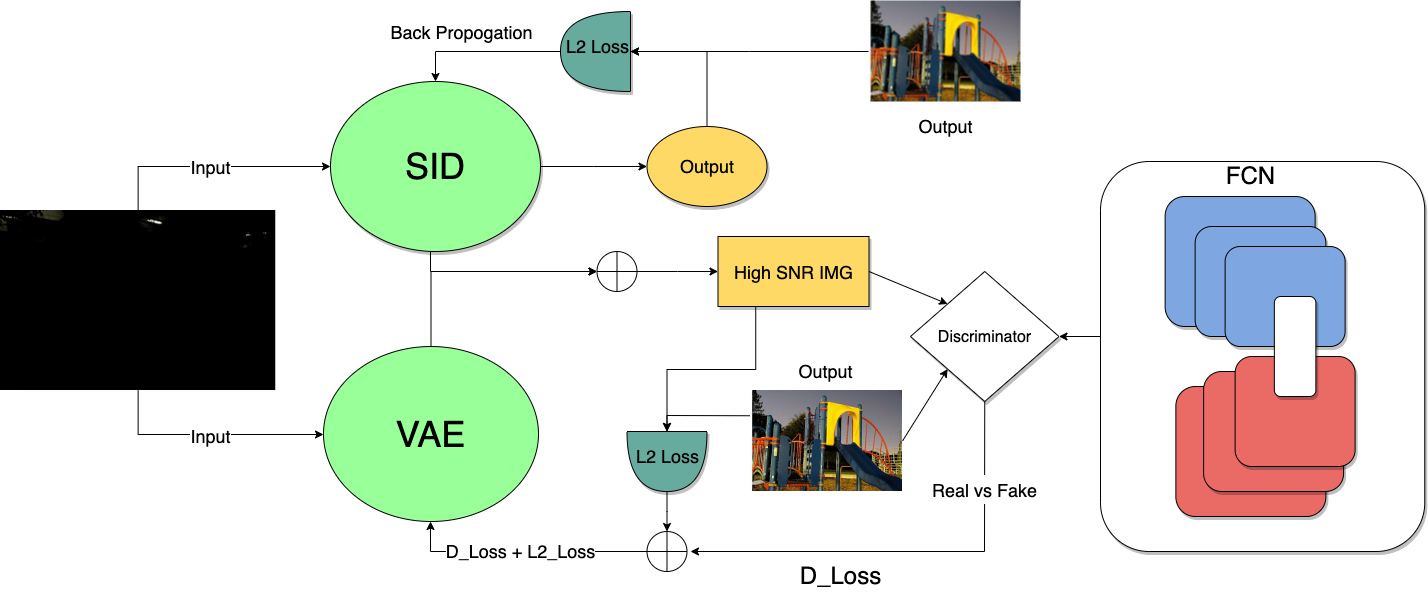
\includegraphics[width=\textwidth]{VAE Diagram.drawio.png} % Replace 'example-image' with the filename of your image
  \caption{Various alternative network architectures were explored and experimented with; however, despite our efforts, we were unable to achieve significantly improved results. Including the VAE-GAN architecture showned above.}
  \label{fig:vae-diagram}
\end{figure*}

\begin{figure*}[t]
  \centering
  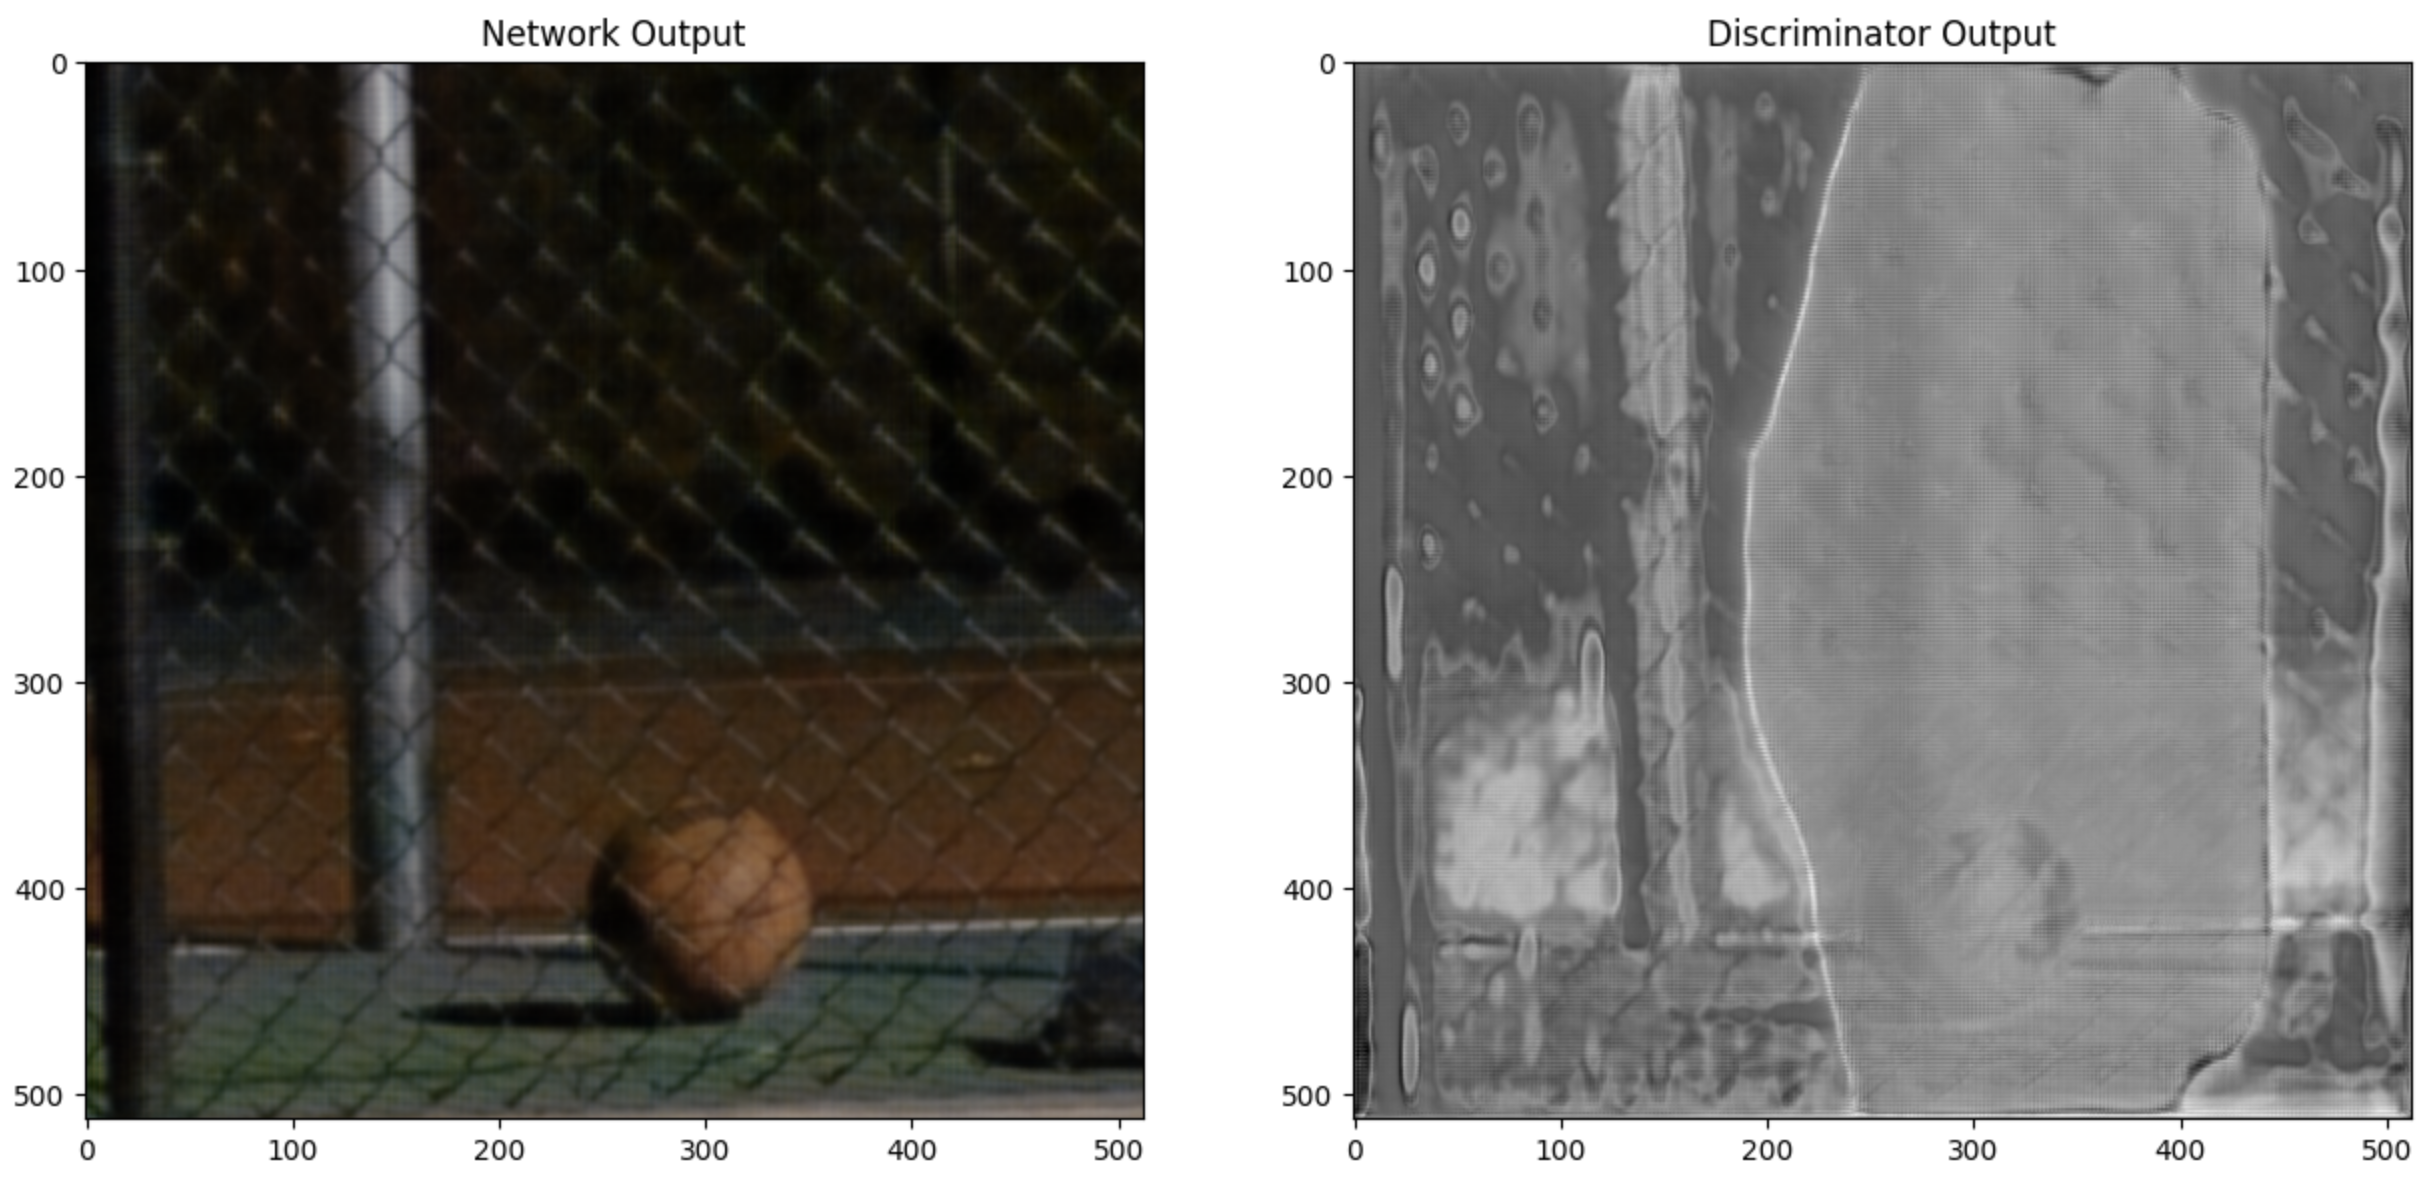
\includegraphics[width=\textwidth]{UnetGAN.png} % Replace 'example-image' with the filename of your image
  \caption{Discriminator network output obtained from the Unet-gan architecture.}
  \label{fig:vae-diagram}
\end{figure*}

Our research question poses some restrictions on the types of network architecture we can choose. When we choose network architecture for our experiments, we not only need to consider whether the network is capable of learning the desired features from inputs but also the network capabilities of handling huge inputs, in our case around 12M pixels. This restriction prevents us to use architectures with any linear layer, as the flattening process will result in variate vector lengths. We stick with UNet because of its capability of handling variable input size without changing the structure, thanks to the non-linear bottleneck. From our experiment result with GAN loss and deeper UNet, this architecture might have reach its capability for our task. We are still actively finding different architectures with similar properties in order to push the upper bounds further. 
%whats next?
%Unet GAN attempts

\section{Contribution}


%UUnet Attempt
\section{Conclusion}
%accomplishments
In our research, we tackled the problem of underexposed images by leveraging the power of the U-net architecture in conjunction with advanced deep learning techniques. The U-Net, a convolutional neural network, is know for its effectiveness in image segmentation tasks. We adapted this architecture to address underexposure by designing a modified U-Net model that performs artistic enhancement and detail recovery. The network was trained on a dataset comprising pairs of underexposed images and their corresponding long-exposure ground truth images.

Moving forward, future work should focus on further refining the proposed model and addressing its limitations. The model's ability to generalize across different camera sensors and lighting conditions should be improved. It is also important to optimize the training process to reduce the computational time require for real-time applications. Furthermore, the developed solution can be extended to handle other challenging image conditions, such as overexposure and low-light video processing. By continuing to advance the field of image recovery from underexposed photographs, we can unlock new possibilites for improving visual perception and analysis in wide range of domains.

\medskip
\printbibliography %Prints bibliography
\end{document}